\documentclass[
	digital,
	oneside,
	table,
	nolot,
	color
]{fithesis3}

\usepackage[
  main=english
]{babel}

\usepackage{paratype}

\thesissetup{
    %date          = \the\year/\the\month/\the\day,
    university    = mu,
    faculty       = fi,
    type          = mgr,
    author        = Radovan Lap\'{a}r,
    gender        = m,
    advisor       = John Smith,
    title         = {thesis},
    TeXtitle      = {Thesis},
    keywords      = {keyword1, keyword2, ...},
    TeXkeywords   = {keyword1, keyword2, \ldots},
    abstract      = {This is the abstract of my thesis, which can
                     span multiple paragraphs.},
    thanks        = {These are the acknowledgements for my thesis, which can
                     span multiple paragraphs.},
    %bib           = example.bib,
}

\usepackage{makeidx}      %% The `makeidx` package contains
\makeindex                %% helper commands for index typesetting.
%% These additional packages are used within the document:
\usepackage{paralist} %% Compact list environments
\usepackage{amsmath}  %% Mathematics
\usepackage{amsthm}
\usepackage{amsfonts}
\usepackage{url}      %% Hyperlinks
\usepackage{markdown} %% Lightweight markup
\usepackage{listings} %% Source code highlighting
\lstset{
  basicstyle      = \ttfamily,%
  identifierstyle = \color{black},%
  keywordstyle    = \color{blue},%
  keywordstyle    = {[2]\color{cyan}},%
  keywordstyle    = {[3]\color{olive}},%
  stringstyle     = \color{teal},%
  commentstyle    = \itshape\color{magenta}}
\usepackage{floatrow} %% Putting captions above tables
\floatsetup[table]{capposition=top}

\setlength{\parskip}{5em}

% custom packages
\usepackage{multicol}
\usepackage{mwe} % new package from Martin scharrer
\usepackage{caption}
\usepackage{wrapfig}

\begin{document}

    \chapter{Introduction}
%\addcontentsline{toc}{chapter}{Introduction}

Public-key cryptography has gained its importance in the late 70's. One of the most commonly used cryptosystems nowadays is RSA. The essential demand on this cryptosystem is security. RSA exists in many variants with different implementations. Each implementation chooses a slightly different approach of generating public and private keys to achieve the right balance between security, efficiency, and randomness. Some implementations are openly known, like OpenSSL, but some other like Microsoft CryptoAPI or Yubikey are not published. With each implementation being different, there is a slight bias introduced in public keys generation, which leads to distinct sample space for different sources. 

These biases can be completely harmless, or they can have serious security impacts. Example of this is a recently discovered flaw in Infineon chips\cite{svenda_2}, which affected more than 50\% of Estonian eIDs. This could potentially lead to forging of e-signatures of the residents. The same chip was also used in Slovak eIDs, albeit with less volume of affected people.

The internet contains a huge amount of dumps of randomly collected RSA public keys from unknown sources. If one could accurately link a particular key to its source, knowing the weakness of this source, he would be able to use specific factorization method to break the public key. We presented the introduction to public cryptosystems and overview of RSA in \autoref{chapter-rsa}.

The aim of this thesis is to further extend the previous research of CROCS\footnote{Centre for Research on Cryptography and Security} team \cite{svenda_1}\cite{svenda_3} lead by RNDr. Petr Švenda, Ph.D. We presented their previous work in \autoref{chapter-prev-work}. Our main goal was to study the usage of different machine learning methods to classify public keys, while specifically focusing on neural networks and comparing them to classic methods like Naive Bayes. The question was how much better they perform, or if they even outperform other machine learning models. We explained neural networks in \autoref{chapter-ml} alongside with all of its terminology used the thesis.

From the CROCS team, we obtained a dataset of more than 100 million public keys from 64 different sources. We performed a detailed analysis of this dataset over particular features mainly focusing on finding non-uniform distribution over its sample space. In \autoref{chapter-dataset} we present the analysis results and the dataset description. During the analysis, we discovered a small bias in the most significant bits of a big number of sources from popular libraries like OpenSSL or Libgcrypt.

As a part of this thesis, we implemented a method to work with this dataset efficiently, analyze and train different machine learning models while focusing on being easily extensible with new models. We described the implementation process in \autoref{chapter-implementation}.

Methodologically, we trained hundreds of neural network models over several generated datasets. We compared and discussed the optimal models. Our results presented in \autoref{chapter-results} show that the neural networks have slightly better overall accuracy when compared to the classical methods like Naive Bayes.

\section{Previous work}
\label{chapter-prev-work}

This thesis serves as an addition to ongoing research on this topic by CROCS team. They have made significant progress in this area already. 

In their first publication\cite{svenda_1}, they generated about 60 million key pairs from 22 open and closed-source libraries and 16 smartcards. Furthermore, they discovered a notable bias in some sources, which could be reflected in the bitmask of the 2nd to 7th most significant bit, second least significant bit and the result of modulus modulo 3. This restricted the sample space of available public keys. For some sources, a specific key was more likely to occur and on the other hand, it could totally dismiss keys from out of its sample space.

Mat\'{u}š Nemec in his Master's thesis\cite{thesis_matus_nemec} presented a complete overview of the provided sources with their properties. He presented the comparison of different generation methods of primes and checked, whether they achieve the demanded level of security.

In the subsequent work, Peter Sekan in his Bachelor's thesis\cite{thesis_sekan} made a clustering analysis based on this mask, which divided the sources into 13 groups. Using a Naive Bayes classifier, he was able to identify sources like PGP SDK 4 FIPS with high probability, while others not at all. He achieved an overall success rate of 33.44 \%. Later in the article\cite{svenda_1}, the rate was increased to 40.34~\%.

The second publication by CROCS team\cite{svenda_3} shows the popularity of the chosen cryptographic libraries in internet-wide TLS scans. They discovered that more than 85\% of all keys originated from OpenSSL library (up to 96\% within GitHub users), followed by the libraries from Microsoft, Libgcrypt, BouncyCastle, and Crypto++. Also, they showed how these libraries got popular in the last seven years. As OpenSSL is by far the most popular network security library nowadays, any bias found in the generation process would affect the majority of keys on the internet.

In the third publication\cite{svenda_2}, they discovered an algorithmic flaw of keys generated by Infineon smartcards, which could be exploited using Coppersmith's attack. Once again, a good classifier for this group would be useful to filter vulnerable keys from an unknown dataset.


    \chapter{Public-Key Cryptosystems}
\label{chapter-rsa}

In this chapter, we will present a basic overview of public-key cryptosystems, focusing mainly on the RSA, the most commonly and widely used public-key cryptosystem.

\subsection*{Private-Key Cryptosystems}

Before 1977 every used cryptosystem was private-key (or symmetric), where both communicating parties Alice and Bob\footnote{in cryptographic terminology, two parties are commonly referred to as Alice and Bob} shared the same secret key. The secret key was then used for encryption and decryption respectively. However, the main issue was how to securely distribute shared secret key between Alice and Bob. Either completely secure channel was used with no eavesdropping possible, or some key exchange method like Diffie-Hellman key exchange \cite{diffie_hellman} was used. The problem of distribution of the private key served as the motivation behind the concept of public-key (asymmetric) cryptosystem invented by Diffie and Hellman \cite{diffie_hellman}. Public-key cryptosystems are undoubtedly the building blocks of modern cryptography and internet security as of today. In practice, we use them basically for any kind of secure transmission of information via internet like money transfers, government communication, secure messaging on social networks and countless others.

\subsection*{Public-Key Cryptosystems}

In a public-key cryptosystem, each user has to generate a pair of private/public key $(d,e)$. Public key $e$ is revealed and used to encrypt messages $m$. Private key $d$ is kept secret and used to decrypt ciphertext $c$. Public-key cryptosystems have the following four properties:

\begin{itemize}

	\item[(a)] $d$ and $e$ are inverse to each other, formally:

$d(e(m)) = m$

	\item[(b)] both $e$ and $d$ are easy to compute

	\item[(c)] it is impossible or at least infeasible to compute $d$ just by knowing the public-key $e$

	\item[(d)] if a message $m$ is first deciphered an then encrypted, the result is the same, formally:
    
$e(d(m)) = m$

\end{itemize}

\noindent
The encryption function $e$ has to meet two necessary requirements:

\begin{itemize}

\item \textit{trap-door one-way function} \cite{trapdoor} - function is easy to compute in one direction, but it is very difficult to compute the inverse of it. Typical examples are prime multiplication vs. prime factorization or power modulo vs. discrete logarithm. Most of the public-key cryptographic protocols are based around these one-way functions.

\item \textit{trap-door one-way permutation} - function is above all also bijective, which means, that $e$ is deterministic 

\end{itemize}

\subsection*{Privacy}

The process of secure data transmission:

\begin{itemize}

\item \textit{encryption} $c = e(m)$ - Alice encrypts the message using Bob's public key, she obtains the ciphertext $c$ which is then transmitted via channel. An eavesdropper can only see this ciphertext which makes no sense to him provided that he cannot crack the system and decrypt the message

\item \textit{decryption} $m = d(c)$ - Bob uses his private key to obtain the original Alice's message

\end{itemize}

\subsection*{Signature}

The problem of one-way authentication or the message signature is another common event appearing in the network communication. Bob wants to have a proof that the message indeed originated from Alice. In this case, Alice supplements the message with its signature. It must be easy for anyone to recognize the signature as authentic, but impossible for anyone other than Alice to produce it. The process of a digital signature is effectively an inverse operation to encryption:

\begin{itemize}

\item \textit{signature} $s = d(m)$ - Alice signs the message using her private key. The signature must be message-dependent, as well as signer-dependent

\item \textit{verification} $m = e(s)$ - Bob uses Alice’s public key to check, whether the message was sent from her

\end{itemize}

\section{RSA cryptosystem}

One of the first public-key as well as the most commonly used cryptosystem today is RSA. It was publicly described by Rivest, Shamir and Adleman (thus RSA) in 1978 \cite{rsa_paper}. RSA gained popularity because of its simplicity as it uses relatively simple power modulo operations. It can be implemented in various ways and over the years many different implementations of this protocol have arisen. It is widely used in the field of software libraries (OpenSSL, Microsoft CryptoAPI, Libcrypt, $\cdots$), cards (Yubikey, Infineon, $\cdots$) or HSM's\footnote{hardware security module}.


\subsection*{Key pair generation}

Every entity that wants to generate a pair of keys is following these steps:

\begin{enumerate}

\item Generate two huge random distinct primes $p$, $q$
\item Compute modulus $n = pq$
\item Choose any public exponent $e$, such that $2 < e < \varphi(n)$\footnote{Euler's totient function, in this case $\varphi(n) = (p-1)(q-1)$} and $e$ is coprime to $\varphi(n)$
\item Compute public exponent $d \equiv e^{-1} \pmod{\varphi(n)}$\footnote{easily computable by Extended Euclidean algorithm}

\end{enumerate}

Detailed key generation process is explained in \cite{thesis_matus_nemec}. The resulted key pair is thus:

\begin{itemize}

\item public key $(n, e)$

\item private key $(d, p, q)$

\end{itemize}

\subsection*{RSA cryptographic primitives}

Every message $m$ can be represented as a positive integer between 0 and $n-1$.\footnote{in case of longer messages we would need to split the message into blocks of integers, where every block would have a value of at most $n-1$} The following cryptographic primitives are present in RSA scheme for message $m$:

\newpage

\begin{itemize}

\item \textit{encryption} $c \equiv m^e \pmod{n}$
\item \textit{decryption} $m \equiv c^d \pmod{n}$
\item \textit{signature} $s \equiv m^d \pmod{n}$
\item \textit{signature verification} $m \equiv s^e \pmod{n}$

\end{itemize}

\noindent
These power modulo operations can be computed very efficiently.

\subsection{Generation bias}

While implementing RSA, many individual sources implement finding candidate primes $p,q$, and public/private exponents $d,e$ differently. Some of them are actively avoiding various properties of primes, which can then lead to the restriction on sample space of available prime numbers:

\begin{itemize}

\item \textit{OpenSSL} is rejecting any candidate, which is congruent to 1 modulo any prime up to 17863 as first reported by Mironov \cite{mironov}

\item smartcard \textit{Infineon JTOP 80K} is generating such primes, which when divided by 11 give a remainder of 1 or 10, by 37 a remainder of 1, 10 or 26 and others

\item some sources like \textit{G\&D SmartCafe 4.x} and \textit{G\&D SmartCafe 6.0} are using only Blum primes\footnote{A prime $p$ is a Blum prime if $p \equiv 3 \pmod{4}$}, which means, that the resulting public key is always congruent to 1

\end{itemize}

These decisions in the process of generation leave significant bias in some sources. When connecting given public-key to its source, one can look at these properties and with high probability differentiate between sources and correctly classify public-key.

We looked at some basic properties for our dataset and found bias in several sources. The full list can be seen in \autoref{appendix-analysis}. These features are used for machine learning classifiers. More details about the dataset can be seen in \autoref{chapter-dataset}.

    \chapter{Neural networks}
\label{chapter-ml}

\section{Artificial neuron}

Artificial neurons, also called perceptrons were developed in the late 1950s and early 1960s, firstly introduced by Rosenblatt in his paper \cite{perceptron}. His idea was to develop a model capable of simulating the activities present in the human brain cell, in order to create artificial intelligence. As it turned out, simulating the brain using such a simple model as the perceptron is impossible. However, later research discovered a considerable potential in the field of classification and regression, which lead to the design of modern artificial neural networks as we know them today.

Perceptron\cite{nn_book} is a simple probabilistic model, which takes several weighted real inputs and produces one real output.

\vspace{3mm}

\begin{figure}[h]
\raggedright
\begin{subfigure}{.35\textwidth}
  \centering
  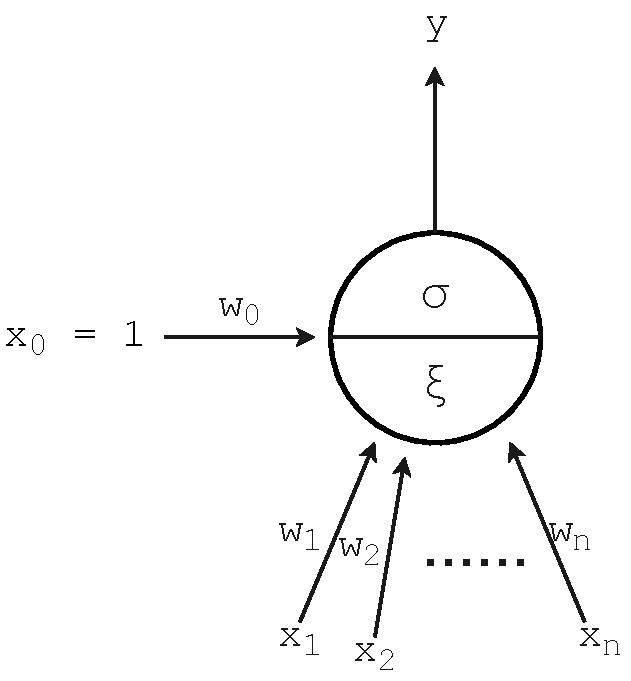
\includegraphics[width=\textwidth]{tex/images/perceptron}
  \caption{Artificial neuron}
\end{subfigure}%
\hfill
\begin{subfigure}{.55\textwidth}
  \centering
  \begin{itemize}

	\item $x_1, \cdots, x_n$ are real \textbf{inputs}
	\item $x_0$ is always equal to 1
	\item $w_0, w_1, \cdots, w_n$ are real \textbf{weights}
	\item $\xi$ is inner \textbf{potential}, \\$\xi = w_0 + \Sigma_{i=1}^n w_i x_i$
	\item $y$ is real \textbf{output} given as \\ $y = \sigma(\xi)$
	\item $\sigma$ is an \textbf{activation function}

	\end{itemize}
\end{subfigure}
\end{figure}

\section{Activation}

An activation function $\sigma: \mathbb{R} \rightarrow \mathbb{R}$ is applied to the inner potential $\xi$, and it defines the output value of perceptron. It introduces a powerful tool into machine learning, and that is \textbf{non-linearity}. Without the activation, the potential by itself is a simple polynomial of a degree of one. That would limit the learning ability of the neural network into being a simple regression model. However, using different activation functions, we can adapt the model to more complicated mappings.

\begin{figure}[h]

\centering
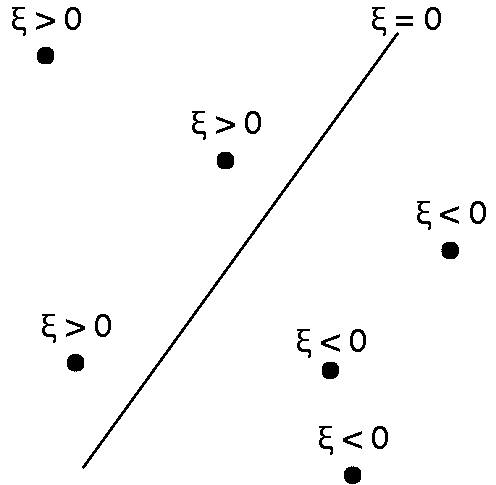
\includegraphics[width=0.45\textwidth]{tex/images/activation-vis}
\caption{Visualization of binary step activation function, which defines a separation hyperplane in n-dimensional space.}
\end{figure}

\noindent
Some desirable properties\cite{wiki:activation} of an activation function include:

\begin{itemize}

\item \textit{non-linearity} - in order to map more complex functions (allows universal function approximations)
\item \textit{continuous differentiability} - the necessity for gradient-based optimization methods
\item \textit{range} - for infinite range, training is generally more efficient
\item \textit{monotonicity} - the error surface associated with a single-layer model is guaranteed to be convex
\item \textit{approximates identity near the origin} - initial weights can be randomized with small differences around the origin

\end{itemize}

\noindent
Here are some examples of activation functions\cite{activation_list}:

\subsection*{Identity}

\begin{figure}[H]
\raggedright
\begin{subfigure}{.25\textwidth}
  \centering
  \[ f(x) = x \]
\end{subfigure}%
\begin{subfigure}{.25\textwidth}
  \centering
  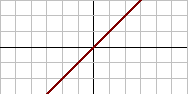
\includegraphics[width=\textwidth]{tex/images/activation/identity}
\end{subfigure}
\end{figure}

\noindent
Effectively remain the potential unchanged. 

\subsection*{Binary step}

\begin{figure}[H]
\raggedright
\begin{subfigure}{.35\textwidth}
  \centering
   \[
f(x) = \begin{cases}
       0 & x < 0 \\
       1 & x \geq 0 \\
     \end{cases} \]
\end{subfigure}%
\begin{subfigure}{.25\textwidth}
  \centering
  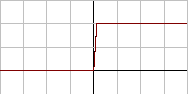
\includegraphics[width=\textwidth]{tex/images/activation/binstep}
\end{subfigure}
\end{figure}

\noindent
Basic activation function, transforms potential into a binary signal. However, this function is not differentiable.
      
\subsection*{Sigmoid}

\begin{figure}[H]
\raggedright
\begin{subfigure}{.28\textwidth}
  \centering
  \[ f(x) = \frac{1}{1 + e^{-x}} \]
\end{subfigure}%
\begin{subfigure}{.25\textwidth}
  \centering
  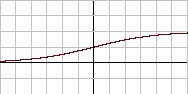
\includegraphics[width=\textwidth]{tex/images/activation/sigmoid}
\end{subfigure}
\end{figure}

\noindent
Smoothened binary step activation function, maps a real value potential into $(0,1)$ range. One of the most popular functions in the ANN's, mainly in the early era of machine learning. It introduces non-linearity. It suffers from vanishing gradient problem\footnote{described in subsection \ref{vanishing_gradient}} and have slow convergence. Furthermore, it is not zero centered, which make optimization harder.
 
\subsection*{TanH}

\begin{figure}[H]
\raggedright
\begin{subfigure}{.5\textwidth}
  \centering
  \[ f(x) = tanh(x) = \frac{(e^x - e^{-x})}{(e^x + e^{(-x)})} \]
\end{subfigure}%
\begin{subfigure}{.25\textwidth}
  \centering
  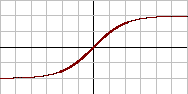
\includegraphics[width=\textwidth]{tex/images/activation/tanh}
\end{subfigure}
\end{figure}

\noindent
Unlike sigmoid, hyperbolic tangent is zero centered. It usually performs better than sigmoid. However, it stills suffers from vanishing gradient problem.

\subsection*{Rectified linear unit (ReLU)}

\begin{figure}[H]
\raggedright
\begin{subfigure}{.35\textwidth}
  \centering
   \[
f(x) = \begin{cases}
       0 & x < 0 \\
       x & x \geq 0 \\
     \end{cases} \]  
\end{subfigure}%
\begin{subfigure}{.25\textwidth}
  \centering
  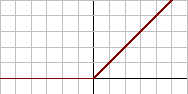
\includegraphics[width=\textwidth]{tex/images/activation/relu}
\end{subfigure}
\end{figure}

\noindent
One of the most popular function in recent years. As opposed to previous ones, it does not have an issue with vanishing gradient. It is simple and efficient. The limitation is that it should only be used within hidden layers of a model, often combined with softmax in the output layer. It turned out to be very useful in deep learning, where traditional activation functions struggle. For example in \cite{relu_faster}, the convolutional network was able to converge six times faster with ReLU, than with tanh.

\subsection*{Leaky ReLU}

\begin{figure}[H]
\raggedright
\begin{subfigure}{.38\textwidth}
  \centering
  \[
f(x) = \begin{cases}
       0.01x & x < 0 \\
       1 & x \geq 0 \\
     \end{cases} \]  
\end{subfigure}%
\begin{subfigure}{.25\textwidth}
  \centering
  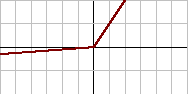
\includegraphics[width=\textwidth]{tex/images/activation/lrelu}
\end{subfigure}
\end{figure}

\noindent
One issue present in ReLU is that it allows the gradient to die off, which is not necessarily a bad thing, though it may result in dead neurons that will never activate on specific data points. To counter this, leaky ReLU's were introduced. To keep the updates alive, they add a small slope into their negative parts (usually with the factor of around 0.01).
   
\subsection*{Randomized ReLU}

\begin{figure}[H]
\raggedright
\begin{subfigure}{.35\textwidth}
  \centering
  \[
f(r, x) = \begin{cases}
       rx & x < 0 \\
       1 & x \geq 0 \\
     \end{cases} \] 
\end{subfigure}%
\begin{subfigure}{.25\textwidth}
  \centering
  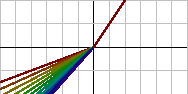
\includegraphics[width=\textwidth]{tex/images/activation/rlrelu}
\end{subfigure}
\end{figure}

\noindent
Another variant of ReLU randomizes the factor in leaky ReLU's.

\subsection*{Softmax}
\label{subsection:softmax}

\begin{figure}[H]
\raggedright
\begin{subfigure}{.25\textwidth}
  \centering
  \[ f(x_j) = \frac{e^{x_j}}{\sum_i e^{x_i}} \]
\end{subfigure}%
\begin{subfigure}{.25\textwidth}
  \centering
  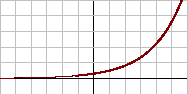
\includegraphics[width=\textwidth]{tex/images/activation/softmax}
\end{subfigure}
\end{figure}

\noindent
Softmax is usually used alongside the ReLU's in the output layer of a deep neural network. It has two nice properties:

\begin{itemize}

\item each value ranges in $[0, 1]$
\item the sum of all values is always 1

\end{itemize}

This is useful when modeling a particular probability distribution. It is used as the estimate of the class distribution for a given input.

\section{Artificial neural network}

Artificial neural network\cite{nn_book} or feed-forward neural network is a directed acyclic graph of artificial neurons organized into several layers, where the following holds:

\begin{itemize}

\item the first layer is called the \textit{input layer}, and the output of neurons is equal to the input vector $\overrightarrow{X}$

\item the last layer is called the \textit{output layer}, and it provides the output $\overrightarrow{Y}$

\item the other layers are called the \textit{hidden layers}

\item outputs of each neuron (except for the output layer) serve as inputs of neurons in the higher layer

\item every two neighboring layers $i$ and $i+1$ make a complete bipartite graph

\item no non-neighboring layers have a connection between them

\end{itemize}

\noindent
In the next sections, we are going to use the following terminology:

\begin{itemize}
  \item every neuron is represented as a distinct natural number (i.e neuron 1, 2, and so forth)
  \item $\xi_i$ is the inner potential of the neuron $i$
  \item $y_i$ is the output of the neuron $i$
  \item $w_{ji}$ is the weight from neuron $i$ to neuron $j$
  \item $j_{\leftarrow}$ is the set of all neurons $i$ such that there exist an edge $w_{ji}$
  \item $j_{\rightarrow}$ is the set of all neurons $i$ such that there exist an edge $w_{ij}$

\end{itemize}

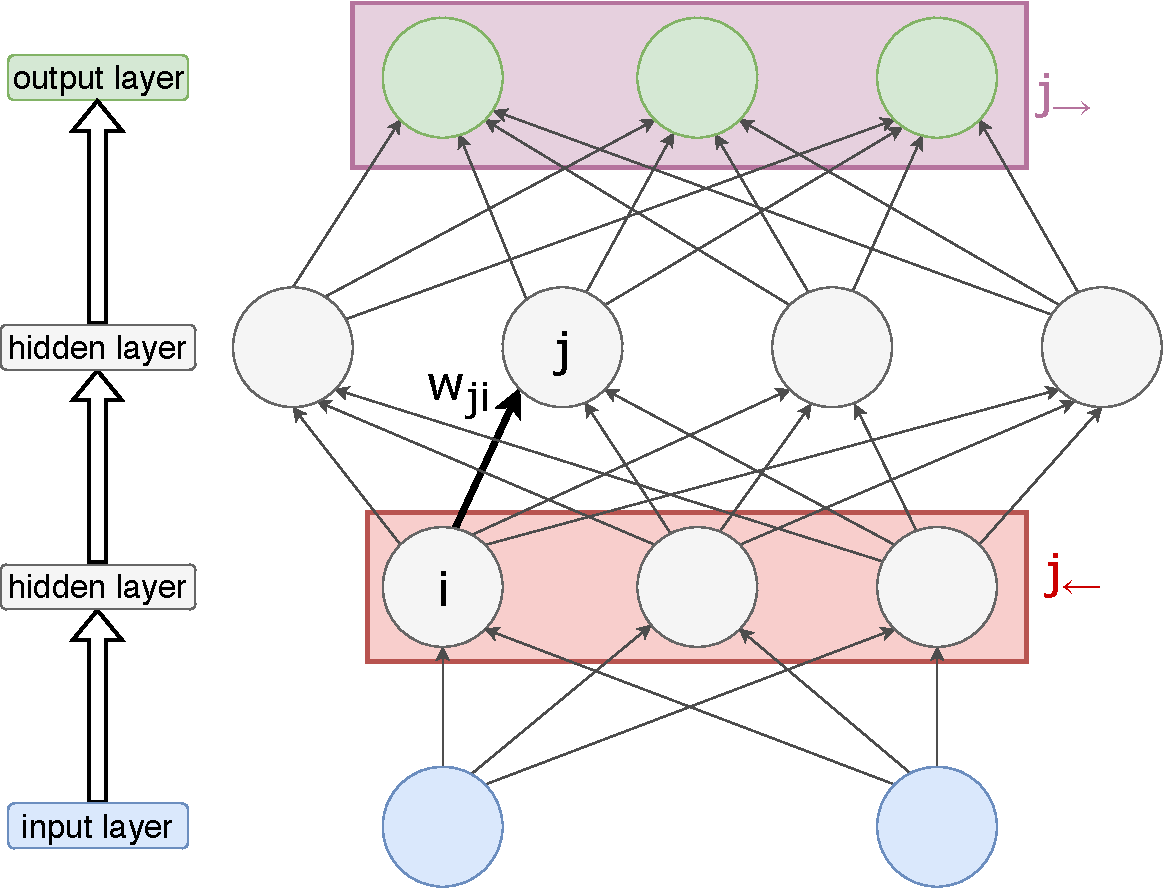
\includegraphics[width=0.8\textwidth]{tex/images/ann}

The neural network is continuously evolving, the states and connections of neurons are changing, weights are adapting. In term of these changes within a period, we can divide the network dynamics into three subcategories:

\begin{itemize}
  \item \textit{organizational} - change in topology
  \item \textit{active} - change in state
  \item \textit{adaptive} - change in configuration
\end{itemize}

\section{Active dynamics}

The values in the input layer are set to the input vector $\overrightarrow{X}$. The forward propagation algorithm is then applied. Starting from the lowest layer, each layer using the output from the previous one updates its neurons. Neuron $j$ updates its inner potential:

$$ \xi_j = w_0 + \sum_{i \in j_{\leftarrow}} w_{ji} y_i $$

The output of neuron $j$ is $y_j = \sigma_j (\xi_j)$. The exception is the input layer, where $y_j = \xi_j$.

\section{Adaptive dynamics}

\textit{Adaptive dynamics} specify the initial configuration of the network and the way, in which the configuration evolves during the training process. Initially are all weights set randomly. In order to update the network weights, we need to define the loss function.

\subsection{Loss function}

At its core, a loss function\cite{loss} is a simple method of evaluating how well the model adapts to the dataset. The higher the loss value is, the more inaccurate the model is. The main goal of the training process is to find the global minima of the loss function. Furthermore, the loss function is differentiable.

Given the set of training data $\tau = \lbrace (\overrightarrow{X_k}, d(\overrightarrow{X_k})) \vert k = 1, \cdots, p \rbrace$, where $\overrightarrow{X_k}$ is a feature, that is fed to the network and $d(\overrightarrow{X_k})$ is a label, that we would like to get as an output from the network.

The loss function is checking the difference between the network's output $\overrightarrow{Y}$ the actual label $d(\overrightarrow{X})$. From now on, we will refer to the output layer as OL in this section.

\subsection*{MSE}

One of the simplest loss function used in machine learning methods is \textit{Mean Squared Error} (of MSE for short):

$$ E(\overrightarrow{w}) = \sum_{k=1}^{p} E_k(\overrightarrow{w}) = \sum_{k=1}^{p} \frac{1}{2} \sum_{j \in \text{OL}} (y_j(\overrightarrow{w}, \overrightarrow{X_k}) - d(\overrightarrow{X_k})_j)^2 $$

\noindent
It is widely used in linear regression analysis.

\subsection*{Cross entropy}

Another very popular loss function, which we used is \textit{cross entropy loss}\cite{cross_entropy}. It is a straightforward modification of a basic likelihood function with logarithms over the probability $p$. It penalizes heavily for being very confident and very wrong. 

In order to transform the output vector $\overrightarrow{Y}$ into the probability distribution $P(\overrightarrow{Y})$ we usually use a softmax activation function in the output layer (as described in section \ref{subsection:softmax}). With the output transformed into a probability vector, we can use the cross entropy:

$$ E(\overrightarrow{w}) =  \sum_{k=1}^{p} E_k(\overrightarrow{w}) = \sum_{k=1}^{p} \sum_{j \in \text{OL}} - d(\overrightarrow{X_k})_j \ln{P(y_j(\overrightarrow{w}, \overrightarrow{X_k}))}$$

\subsection{Gradient descent and backpropagation}

Stochastic gradient descent\cite{deep_learning_SGD} and its variants are probably the most used optimization algorithms for machine learning in general. To update weights according to the given loss function, we need to compute the gradient at any given point on the function in the hyperplane. The gradient vector points towards the closest local minimum. It is the direction in which we want to update our weights.

The learning algorithm is computing the sequence of weight vectors $\overrightarrow{w}^{(0)}, \overrightarrow{w}^{(1)}, \overrightarrow{w}^{(2)}, \cdots$, where:

\begin{itemize}

\item $\overrightarrow{w}^{(0)}$ is the initial vector set randomly (usually weights close to 0)
\item in the $(i+1)$-th step is $\overrightarrow{w}^{(t+1)}$ computed as:

\begin{flalign}
\notag w_{ji} & = w_{ji}^{(t)} + \Delta w_{ji}^{(t)} & \\
\notag \Delta w_{ji}^{(t)} & = - \epsilon(t) \frac{\partial E}{\partial w_{ji}}(\overrightarrow{w}^{(t)}) & 
\end{flalign}

\item $\Delta w_{ji}^{(t)}$ is the weight difference in the step $(t+1)$ and $0 < \epsilon(t) < 1$ is the learning rate in the step $(t+1)$

\begin{flalign}
\notag \frac{\partial E}{\partial w_{ji}} & = \sum_{k=1}^p  \frac{\partial E_k}{\partial w_{ji}} & \\
\notag \frac{\partial E_k}{\partial w_{ji}} & = \frac{\partial E_k}{\partial y_j} \cdot \sigma_{j}^{'}(\xi_j) \cdot y_i & 
\end{flalign}

\begin{flalign}
\notag \frac{\partial E_k}{\partial y_j} &  = 
     \begin{cases}
       y_j - d(\overrightarrow{X_k})_j & \quad\text{for } j \in \text{ OL} \\
       \sum_{r \in j^{\rightarrow}} \frac{\partial E_k}{\partial y_r} \cdot \sigma_{r}^{'}(\xi_r) \cdot w_{rj} & \quad\text{otherwise} \\
     \end{cases} &
\end{flalign}

\end{itemize}

\noindent
While the feed-forward phase was evaluated from the input layer towards the output layer, the weight update is done in the different direction. Starting from the output layer, we are using the partial derivatives from the layer above to evaluate the current layer. This process is also known as \textit{backpropagation}.

There are two general types of weight update algorithms:

\subsection*{Batch algorithm}

It is the approach described above. It takes a batch of data points in each and computes only one weight update for all of these points together. The advantages include:

\begin{itemize}

\item the direction of the descent is identical to the gradient descent vector
\item parallelism is easy to implement - data point losses can be computed secludedly

\end{itemize}

\noindent
The problems of a batch algorithm:

\begin{itemize}

\item memory consumption
\item redundant data do not add any information to the gradient
\item is more likely to end up in some local minimum than the online algorithm

\end{itemize}

\subsection*{Online (stochastic) algorithm}

An online algorithm is essentially a batch algorithm, where batch consists of only one data point\footnote{point can be taken deterministically or at random (thus stochastic)}. Instead of the whole batch, we update the weight for each data point:

$$ \Delta w_{ji}^{(t)} = - \epsilon(t) \frac{\partial E_k}{\partial w_{ji}}(\overrightarrow{w}^{(t)}) $$

\noindent
Therefore it is not taking the path of gradient descent exactly, but rather "zigzag" alongside the gradient descent vector. The advantages include:

\begin{itemize}

\item it has a better chance of escaping the local minimum than batch algorithm
\item less memory consumption
\item faster (especially on redundant data)

\end{itemize}

\noindent
The problems of an online algorithm:

\begin{itemize}

\item not suitable for parallelism
\item can behave weirdly, because it is not taking the direct path to minimum

\end{itemize}

\section{Issues}

There are widely known issues when working with neural networks, which have to be taken into consideration when working with models. In this section, we will mention just a couple, which we encountered and had to deal with.

\subsection{Dataset split}

Very simple, but very crucial mechanism used in machine learning is to define three separate sets (\textit{train}, \textit{valid} and \textit{test}). These sets have to be disjoint. It is necessary to use \textit{valid} set during the training process and different \textit{test} set for model evaluation, once the model is trained. The reason behind is that always the model will have a slight bias towards the \textit{valid} test compared to the independent \textit{test} set.

\subsection{Vanishing gradient problem}

\label{vanishing_gradient}

The \textit{vanishing gradient problem}\cite{vanishing_gradient} is a difficulty found in training ANN's. The problem is, that in some cases the gradient will be vanishingly small with the impact on weight update. It gets more apparent with many-layered feedforward networks as well as with recurrent networks. Activation functions such as \textit{hyperbolic tangent} and \textit{sigmoid} suffer from vanishing gradient, while others like ReLU or Leaky ReLU do not.

\section{Model evaluation}
\label{nn-metrics}

After the training process, a huge emphasis is put into the model evaluation. With the incorrect evaluation methods, even the poorly trained model can have a good overall score. Several factors have to be taken into consideration like the uneven distribution of data classes, false negatives, and false positives or the classification interchanging between two groups.

\subsection{Confusion matrix}

In the field of machine learning and specifically the problem of statistical classification, a \textit{confusion matrix}\cite{conf_matrix} is a two-dimensional matrix $n \times n$, where $n$ is the number of classes. Each row of the matrix represents the instances in a predicted class while each column represents the instances in an actual class. It is the most verbose output of the evaluation. We can see the wrongly classified classes, but also the classes which the model misclassified into. 

\begin{figure}[h]
\centering
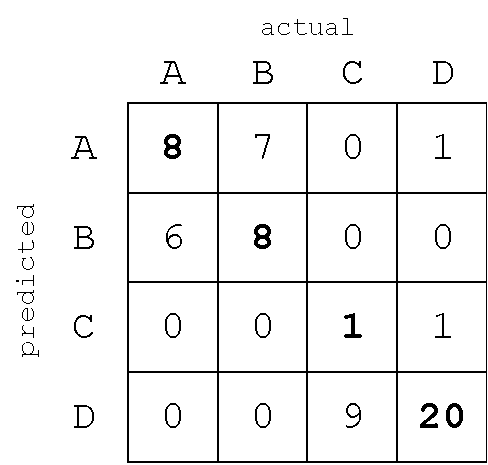
\includegraphics[width=0.37\textwidth]{tex/images/conf_matrix}
\caption{Example of a classification matrix.}
\label{conf_matrix}
\end{figure}

\noindent
In Figure \ref{conf_matrix}, we can see the classification matrix for four classes. The correctly classified cases lie on the main diagonal. Several observations about our model can be seen. First of all, our model almost always misclassifies class \textit{C} as class \textit{D}. Furthermore, the model has difficulties distinguishing between classes \textit{A} and \textit{B} (it would be a good idea to merge these classes).

\subsection{Metrics}

There are four standard metrics \cite{nn-metrics} for model evaluation: \textbf{accuracy}, \textbf{precision}, \textbf{recall}, and \textbf{f1}. Apart from the standard metrics accuracy, the other metrics represent the cost of having false positives and false negatives. Let us take a simple binary confusion matrix:

\begin{table}[h]
\centering
\begin{tabular}{|r|c c|}

\hline 
& $A$ & $\neg A$ \\
\hline 
$A$ & TP & FP \\
$\neg A$ & FN & TN\footnotemark\\

\hline

\end{tabular}

\end{table}

\footnotetext{true positive / false positive / false negative / true negative}

\noindent
We define the four metrics as followed:

\begin{align*}
\textit{accuracy } & = \frac{TP + TN}{TP + FP + FN + TN} & \\
\textit{precision } & = \frac{TP}{TP + FP} & \\
\textit{recall } & = \frac{TP}{TP + FN} & \\
\textit{F1 } & = \frac{2 \times \textit{ precision } \times \textit{ recall}}{\textit{precision } + \textit{ recall}} &
\end{align*}

\begin{itemize}

\item \textbf{accuraccy} - is the standard metric for classifiers, we take the ratio of correctly classified data to the whole dataset. The problem with accuracy is, that it suffers from unbalanced datasets, where the bigger groups can artificially increase accuracy.

\item \textbf{precision} - talks about how precise the model is out of positive predictions and how many are actual positives. It is useful to use when the cost of false positive is high.

\item \textbf{recall} - works the other way around, where we calculate how many of positives are really true positives and not just false negatives. It is useful to use when the cost of false negative is high.

\item \textbf{f1 score} - is a balance between precision and recall and serves as an alternative to the accuracy

\end{itemize}

\section{Grid search}
\label{section-grid-search}

In this thesis, we used the method called \textbf{grid search}\cite{grid-search}. When there are a couple of hyperparameters, the common practice
is to perform a grid search. For each hyperparameter, the user selects a
small finite set of possible values to explore. The grid search algorithm
then trains models for every joint specification of hyperparameter
values in the Cartesian product of the set of values for individual
hyperparameters. The experiment then yields the best model and hyperparameter choice. 





    \chapter{Dataset}
\label{chapter-dataset}

For this thesis, we were provided with the dataset consisting of more than 30 sources collected from different software libraries, hardware authentication devices (or cards) and HSM's\footnote{Hardware security modules}. 
Some of the software libraries had the option of so-called FIPS module, which is a security standard, that put some requirements on generated primes and their distribution, namely available in \textit{PGP SDK 4}, \textit{Libgcrypt} and \textit{OpenSSL}. Furthermore, every source had one or more development versions. 

Considering both of these options, we split our dataset into 64 distinct sources based on their version and whether or not they had the FIPS module activated when generating primes. Every source was represented by a couple of CSV files, with fields $n, e, d, p, q$ and $t$ (time of generation). Three key lengths were present (512b, 1024b and 2048b), with most of the data originated from 512b or 1024b.

All in all, a total of more than 146 million keys were collected with roughly 75.5 million of 512b and 65.4 million of 1024b keys. These two datasets were used for machine learning and preparing classification models. A complete overview of the dataset can be seen in Appendix \ref{appendix-dataset}.

In the article by CROCS lab\cite{svenda_1}, different sources were merged into 13 disjoint groups using clustering on the mask of 9 selected bits. Using the naive Bayes classifier, they were able to classify a random sample of keys with the accuracy of 40.34 \%. Therefore, in this thesis, we tried to pick up on these results and further extend the accuracy by using other classifiers while focusing specifically on neural networks.

\section{Dataset analysis}

\label{chapter-analysis}

Before attempting to create a working classifier, the analysis of the dataset and subsequent feature engineering was necessary. We scanned the whole dataset, extracting features from public product $n$. We focused mainly on the bit value on every position and the remainder when divided by a specific number. With every feature, we counted the relative frequency of every possible value. Because of the huge number of keys, we needed to run this analysis distributively on Metacentrum\footnote{distributed cloud computing over CESTNET}.

\subsection{Modular analysis}

As in the full CROCS report\cite{svenda_full}, we did a similar analysis on the full dataset. With every key, we computed a modulo over first 30 natural numbers, starting with 3, while focusing mainly on prime numbers. We were looking for any irregularities in distribution of the remainders. Specifically, with prime numbers $p$, the remainder should be uniformly distributed between 1 and $p-1$. Several sources showed bias, namely:

\begin{itemize}

\item \textit{mod 3} - sources 2,3 (G\&D SmartCafe 4.x and 6.0), 11-14 (OpenSSL without FIPS module) and 19, 20, 21 (NXP J2D081, NXP J2E145G, YubiKey NEO) were always giving a remainder of 1.

\item \textit{mod 4} - sources 1, 2, 3 (G\&D SmartCafe) 4 (GNU Crypto 2.0.1) 6, 7, 8, 9 (NXP J2A*, NXPJ3A*, NXP JCOP 41 V2.2.1), 10 (Oberthur Cosmo Dual 72K) and 19, 20, 21 were always giving a remainder of 1. Sources that were giving a remainder of 1 modulo 3 and 4 are using Blum integers.

\item \textit{module 11} - sources 16, 17, 18 (Infineon, Yubikey and Yubikey Nano) were giving only remainders of 1 or 10. Sources 11, 12, 13, 14, 19, 20 had slight bias towards the remainder of 1.

\end{itemize}

\noindent
Full results of modular analysis can be seen in Appendix \ref{appendix-modular-analysis}.

\subsection{Bit analysis}

Another analysis focused on full bit analysis. Similarly, as in the previous one, we computed the relative frequency (or probability of 0) on every bit position with each source. This kind of analysis took a more significant amount of time and needed to be computed distributively. It took a couple of hours compared to the estimated time of up to one week when computing on the local machine. The analysis showed a significant bias in the first 6 most significant bits, mostly:

\begin{itemize}

\item \textbf{1st MSB} was always 1 (for bit length padding) with one exception of source 15 (PGP SDK FIPS 4), which contained a majority of its keys with shorter bit length.

\item \textbf{2nd - 4th MSB} could distinguish a lot of groups (i.e. 16-18 or 1-3), because of wider probability distribution.

\item \textbf{5th - 6th MSB} still had slight bias in probability distribution for some groups (4, 19-21, 31-40)

\item \textbf{2nd LSB} could distinguish mostly groups that were using Blum primes (1-4, 6-10, 19-21)

\end{itemize}

\noindent
Full results of bit analysis can be seen in Appendix \ref{appendix-bit-analysis}.

\subsection{Feature engineering}

\label{feature-engineering}

Based on the previous analysis we extracted the following features from the public key to feed to the network:

\begin{itemize}

\item all moduli remainders up to 30 represented as binary vector\footnote{For example for $x \equiv 1 \pmod{5}$, the feature vector is $(1,0,0,0)$, $x \equiv 2 \pmod{5}$ - $(0,1,0,0)$, $\cdots$}

\item The key itself

\end{itemize}

\noindent
The performance of the network was similar regardless of using the full key, or just the biased bits.

\subsection{Source grouping}
If we look closely on the full analysis in Appendix \ref{appendix-analysis}, we can see that based on the feature engineering we can natively group sources, that share the distribution. We obtain 13 groups\footnote{Same grouping was obtained by cluster analysis in \cite{svenda_1}}:

\vspace{5mm}

\noindent
\begin{tabular}{|r|l||r|l||r|l|}

\hline

\textbf{G1} & 1 & \textbf{G6} & 10 & \textbf{G10} & 19, 20, 21 \\
\textbf{G2} & 2, 3 & \textbf{G7} & 11, 12, 13, 14 & \textbf{G11} & 22 - 29 \\
\textbf{G3} & 4 & \textbf{G8} & 15 & \textbf{G12} & 30 - 40 \\
\textbf{G4} & 5 & \textbf{G9} & 16, 17, 18 & \textbf{G13} & 41 - 64 \\
\textbf{G5} & 6, 7, 8, 9 & & & & \\

\hline

\end{tabular}

    \chapter{Notes}

\textbf{PIPELINE}
\begin{itemize}

\item dataset
\item key batch available
\item set of scripts over dataset
\item features from paper [Svenda2]
\item analysis of dataset (distributions of moduli)
\item feature engineering
\item different models (Scikit-learn models, keras models)
\item better results than svenda
\item needed optimization (usage of python generators) to be able to work with huge dataset in memory
\item this leads to better usage o metacentrum as well
\item next step was to split up the dataset into sources only and check this
\item split and merge groups (especially G13)
\item g15 binary classifier
\item yubikey binary classifier (same chip for infineon/yubikey)
\item sampling of training dataset 
\item Scripts to work with dataset (url)
\item preprocessed dataset (url) and final models git
\item every used model theory (multilayer perceptron, binary classifier, deep learning)
\item pandas, keras docs
\item similar work (mention Svenda papers, THESIS1, THESIS2)

\item implementation chapter (with dataset section)
\item metacentrum


\end{itemize}

\end{document}